\section{Conclusions}
% 
% 
\subsection{Results Analysis}
\subsubsection*{Unveiling Team Prowess Through Fourier Transform Analysis}
\paragraph{Historical data serves as a manifestation of a team's capabilities. Therefore, we consider each set of data from the past 15 years of the English Premier League as a unique signal. By applying Fourier transforms in both the time and frequency domains, we aim to extract hidden information from these historical datasets, treating each team's performance as a distinctive signal. We employ feature extraction formulas to analyze these signals, attempting to unveil latent information that reflects the teams' strengths. This approach helps delve into patterns and trends in a team's past performances, providing a more comprehensive understanding of their athletic prowess.}
% 
% 
% 
\begin{figure}[H]
    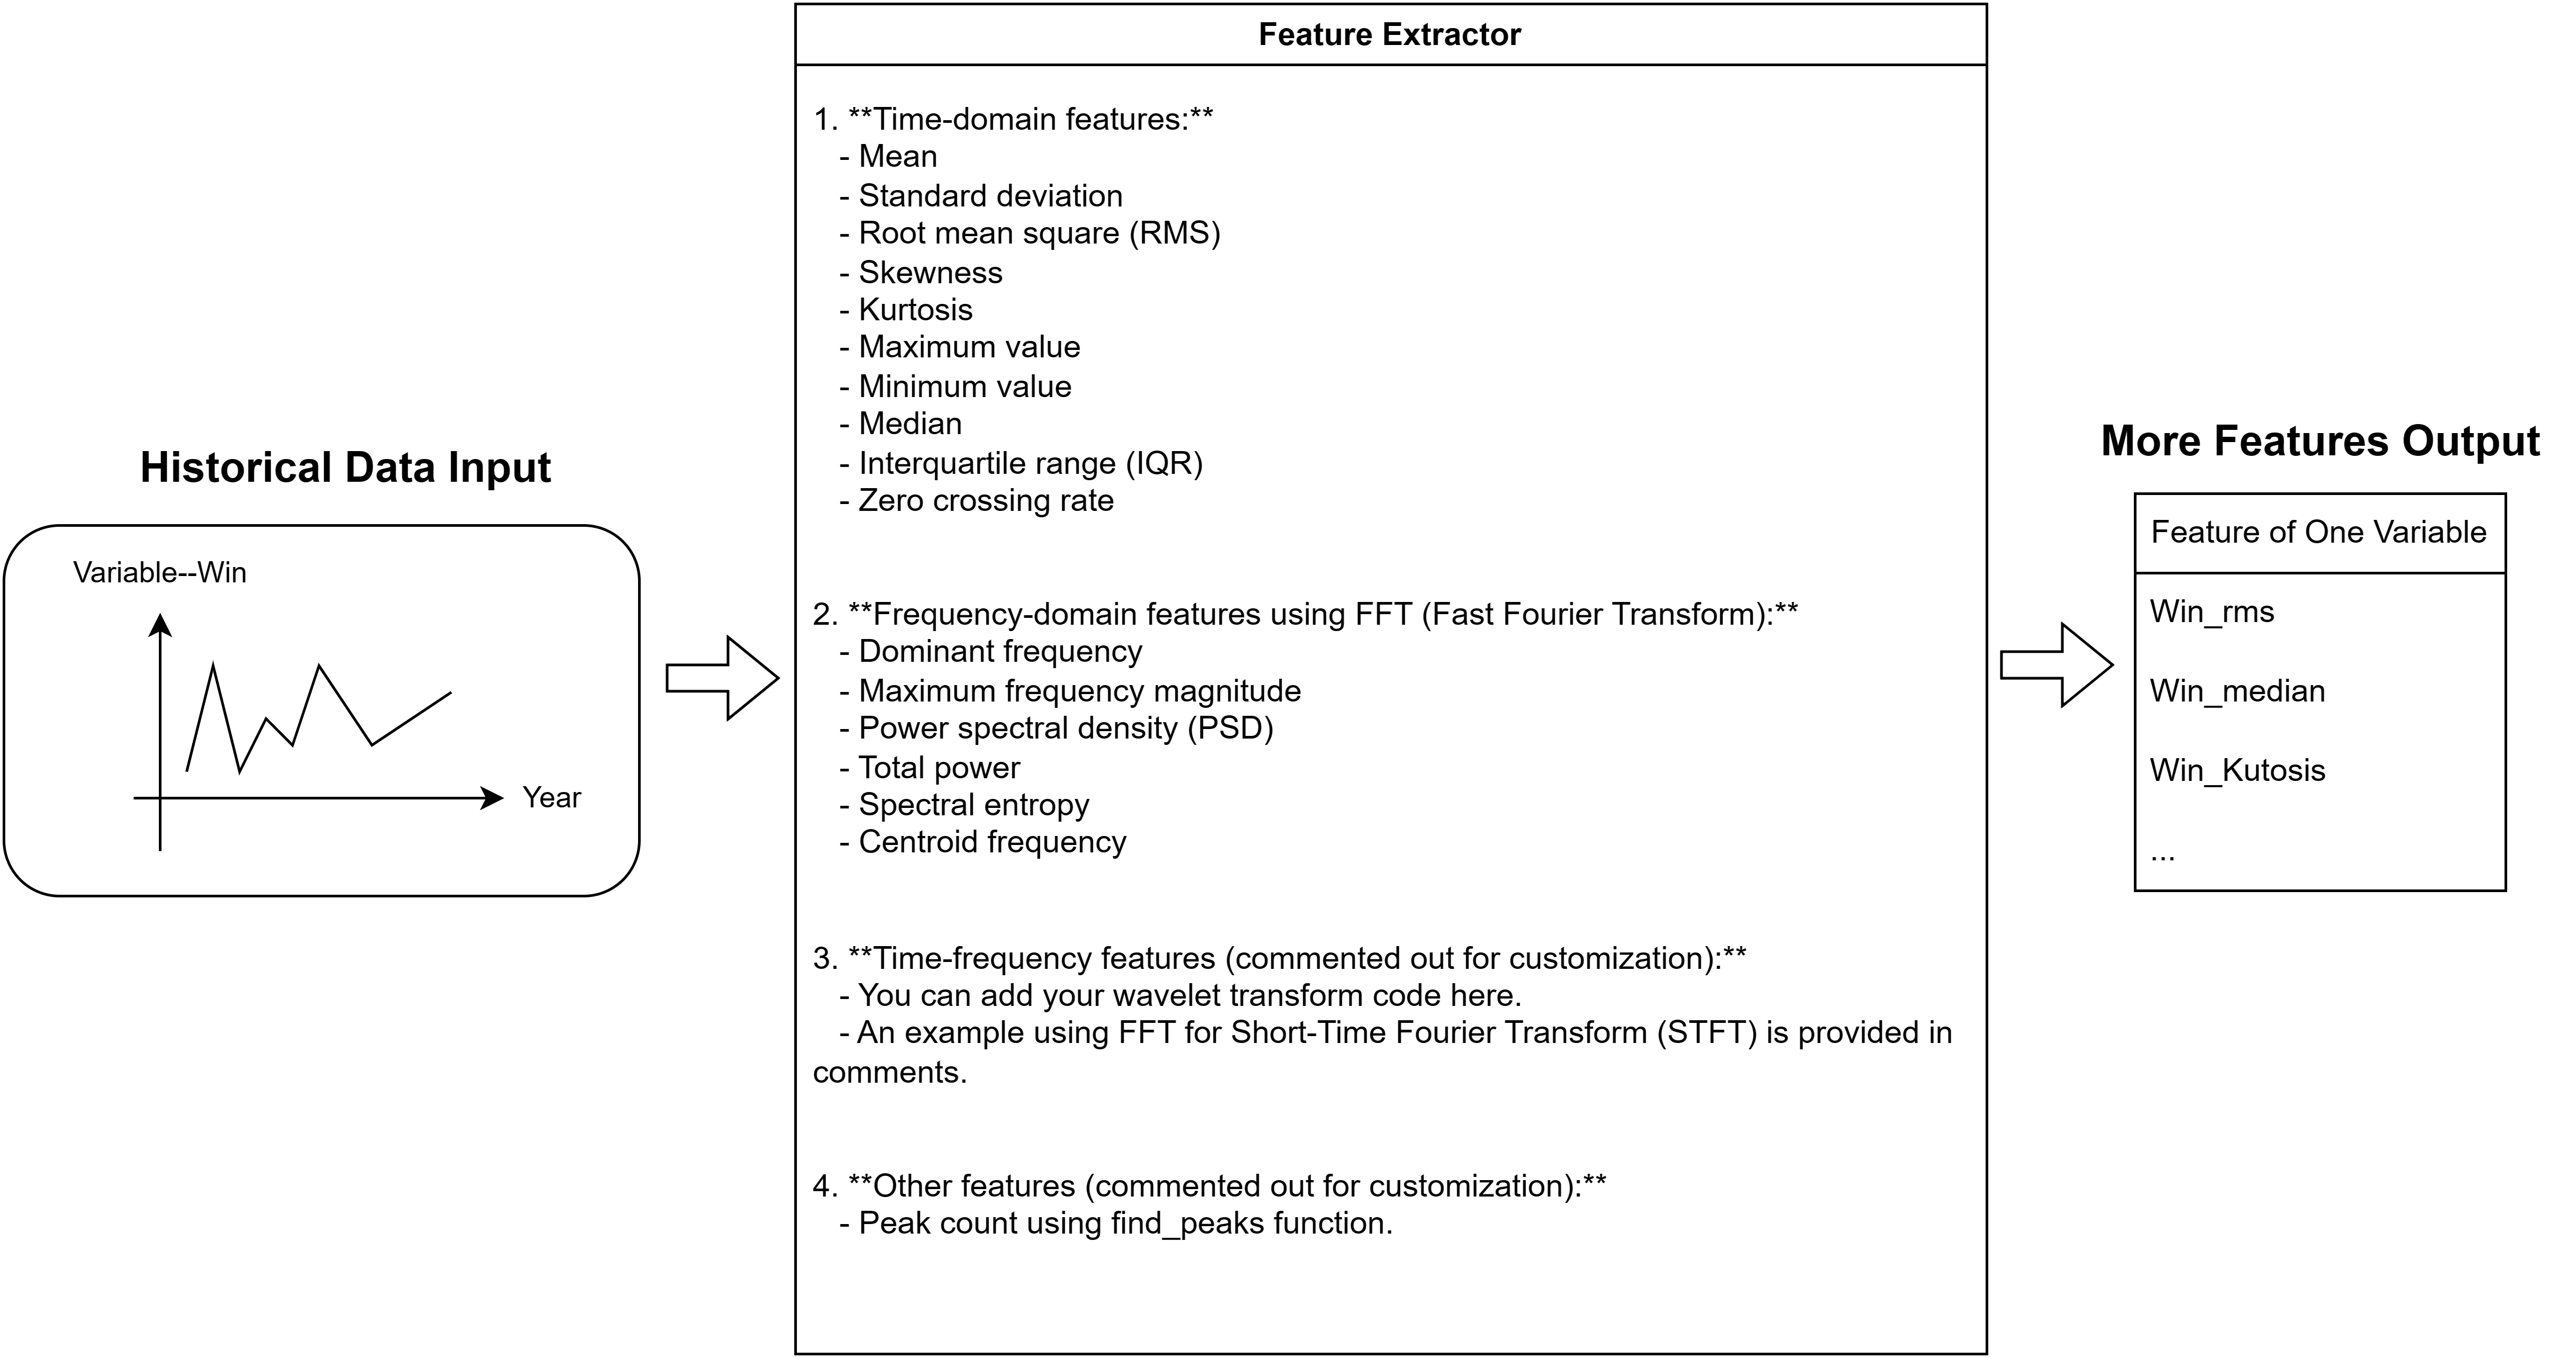
\includegraphics[width=\textwidth]{pic/feature.png}
    \caption{Feature Extraction}
    % \label{fig:DataGrab}
\end{figure}
% 
% 
% 
% 
\paragraph{Our initial dataset comprises only 9 columns from the 2023-24 season. Through feature extraction on historical season data, we have expanded the dataset to include 121 columns. This provides us with greater flexibility for the upcoming steps of correlation analysis and PCA.}